\section{Introduction}
\label{sec:intro}

In this paper we seek to analyze the past and current state of Namecoin. We look at the primary two uses of Namecoin, a distributed DNS and OpenName, a distributed identity system. The vast majority of registered names in Namecoin fall under the DNS. However the  majority of real Namecoin usage comes from OpenName. This is due to the extremely high rate of name squatting within Namecoin. We quantitatively and qualitatively analyze the behavior of squatters within the Namecoin ecosystem and how they interact with regular users. Then we explore strategies suggested among the Namecoin community for preventing squatting and estimate what kind of effect these anti-squatting strategies would have on Namecoin. Finally we discuss the best ways Namecoin can be used in the future.

\subsection{Background}
<<<<<<< HEAD
Namecoin is an alternative cryptocurrency modeled after Bitcoin. Furthermore, it is the first altcoin in the sense that it was the first to create its own blockchain, separate from Bitcoin's. Namecoin shares many similarities with Bitcoin, including the same method for proof of work, the same coin cap, the same block creation time, and all of the same transaction operations. The additional feature of Namecoin, as opposed to Bitcoin, is that it has built-in support for posting and updating name/value pairs (same as the more traditional key/value store) to its blockchain. The values associated with names can be updated by their owners and ownership of names can be transferred between users. The name/value store is a general data structure which can be used to implement a diverse array of systems. Namecoin originally came around after discussions about a BitDNS protocol using a blockchain to manage a domain name lookup service. The idea behind this is that a central authority managing domain names, such as ICANN, requires too much trust in a single entity. Having centralization like this allows the central authority to censor content at will. It also provides a single point of failure, which can go down, or can be forced by an oppressive government to censor information. It is more ideal to instead have a decentralized Domain Name System (DNS) and using a blockchain data store can provide just that.

The name/value store built into Namecoin can provide this lookup service by having people register names representing domain names, and values representing the locations on the internet a browser should go to view a website. The protocol was made very general so that it could also be useful for any system in which a name/value data store is necessary. In order to support multiple uses at the same time, the Namecoin names are broken up into different namespaces. When registering a name, an individual will identify the namespace and the desired name, separated by a slash. The namespace used for DNS is denominated by d/<name>. Since the genesis of Namcoin it has been used for a variety of services other than just DNS. In particular, the online identity system OneName utilizes the Namecoin name/value store in the namespace u/<name>. Namecoin adds this data store by offering three additional script operations to the Bitcoin scripting language: NAME\_NEW, NAME\_FIRSTUPDATE and NAME\_UPDATE. Registering a name is covered in depth in the registration protocol section. 

The reason  why a blockchain makes such a good decentralized data storage system is that everyone who uses the system will have the same blockchain (and hence the same data) stored on their machine. The reason why everyone has the same blockchain returns us to Bitcoin and the concept of proof-of-work. Essentially everyone agrees on the blockchain that is the longest (that has the most proof-of-work). The proof-of-work is what makes it computationally infeasible for an adversary to trick someone into believing a false blockchain. The value and stability of the system are directly related to the amount of proof-of-work involved in the calculations of the blocks because this work is what keeps the data distributed and secure. For both Bitcoin and Namecoin, the proof-of-work is shown by calculating the hash of a new block and a random nonce over and over until the calculated hash has a certain number of leading zeros. The number of leading zeros required by the hash is referred to as the difficulty threshold. 
    Namecoin enjoys a very high difficulty threshold for the proof of work. Namecoin is able to do this because it supports merge mining with Bitcoin. This allows miners who are mining Bitcoin to also mine Namecoin at the same time with essentially no extra work for the miner. Essentially, this is because the miner is using their computational power to solve a cryptographic puzzle that satisfies the proof-of-work for both blockchains at the same time. This is advantageous for the miners because they are rewarded with coins from both systems, and helps Namecoin because it gives the Namecoin network a vastly increased amount of hash power over what it would have if it did not support merged mining. The high hash power and difficulty of the cryptographic challenge on the Namecoin network increases the stability of the system, providing resilience to a 51\% attack and other threatening behaviours from malicious miners. 
=======

Namecoin is an alternative cryptocurrency modeled after Bitcoin\cite{nakamoto2008bitcoin}. Furthermore, it is the first altcoin in the sense that it was the first to create its own blockchain, separate from Bitcoin's. Namecoin shares many similarities with Bitcoin, including the same method for proof of work, the same coin cap, the same block creation time, and all of the same transaction operations. The additional feature of Namecoin is that it has built-in support for posting and updating name/value pairs (same as the more traditional key/value store) to its blockchain. A key in Namecoin is generally referred to as a ``name''. The values associated with names can be updated by their owners and ownership of names can be transferred between users. The name/value store is a general data structure which can be used to implement a diverse array of systems.

Namecoin came to be after discussions about a BitDNS\cite{bitdns} protocol using a blockchain to manage a domain name lookup service. The idea behind this is that a central authority managing domain names, such as ICANN, requires too much trust in a single entity. Having a centralized name system allows the central authority to censor content at will. It also provides a single point of failure, which can become unavailable, or can be forced by a government to censor information. A decentralized system can be more robust in the face of these deficits.

The name/value store built into Namecoin can provide this lookup service by having people register names representing domain names, and values representing the locations on the internet a browser should go to view a website. The protocol was made very general so that it could also be useful for any system in which a name/value data store is necessary. In order to support multiple uses at the same time, the Namecoin names are broken up into different namespaces. When registering a name, an individual will identify the namespace and the desired name, separated by a slash. The namespace used for DNS is denominated by d/<name>. Since the genesis of Namecoin it has been used for a variety of services other than just DNS. In particular, the online identity system OneName utilizes the Namecoin name/value store in the namespace u/<name>. Namecoin adds this data store by offering three additional script operations to the Bitcoin scripting language: NAME\_NEW, NAME\_FIRSTUPDATE and NAME\_UPDATE. Registering a name is covered in depth in the registration protocol section. 

The reason  why a blockchain makes such a good decentralized data storage system is that everyone who uses the system will have the same blockchain (and hence the same data) stored on their machine. The reason why everyone has the same blockchain returns us to Bitcoin and the concept of proof-of-work. Essentially everyone agrees on the blockchain that is the longest (that has the most proof-of-work). The proof-of-work is what makes it computationally infeasible for an adversary to trick someone into believing a false blockchain. The value and stability of the system are directly related to the amount of proof-of-work involved in the calculations of the blocks because this work is what keeps the data distributed and secure. For both Bitcoin and Namecoin, the proof-of-work is shown by calculating the hash of a new block and a random nonce over and over until the calculated hash has a certain number of leading zeros. The number of leading zeros required by the hash is referred to as the difficulty threshold. 

Namecoin enjoys a very high difficulty threshold for the proof of work. Namecoin is able to do this because it supports merge mining with Bitcoin. This allows miners who are mining Bitcoin to also mine Namecoin at the same time with essentially no extra work for the miner. Essentially, this is because the miner is using their computational power to solve a cryptographic puzzle that satisfies the proof-of-work for both blockchains at the same time. This is advantageous for the miners because they are rewarded with coins from both systems, and helps Namecoin because it gives the Namecoin network a vastly increased amount of hash power over what it would have if it did not support merged mining. The high hash power and difficulty of the cryptographic challenge on the Namecoin network increases the stability of the system, providing resilience to a 51\% attack and other threatening behaviours from malicious miners. 
>>>>>>> bd18d8645dfc010e20313dbb88297cc5a6b98163


\subsection{Registration Protocol}
The feature that separates Namecoin from Bitcoin is that Namecoin can be used to register name/value pairs that can be stored in the blockchain and traded amongst individuals. This registration is done using the three script operations exclusive to Namecoin. In order to understand the registration process, we think it is helpful to walk through the registration process of a name, roughly following Figure \ref{fig:registration}. To start, the user will need to select a coin to use, because by the end of this entire process the user will have a 0.01 NMC token (or special coin) that represents a name, whose value can be changed by whoever holds the special coin. The next step to register a name is to make a transaction that uses the NAME\_NEW  operation. Using NAME\_NEW, a user can indicate an interest in a new name for a name/value pair by posting a hash of the desired name concatenated with a random nonce. Specifically, by ``posting a hash'', we mean that in the scriptPubKey of a special transaction there will be some additional arguments, including this hash. To do this, the user will create said transaction with the 0.01 NMC (and enough other funds to cover a transaction fee) as input, and will send the special coin to an address they control. As mentioned, the output scriptPubKey will contain the usual signature locking operations, following the additional NAME\_NEW operation and arguments.

\begin{figure*}
  \centering
  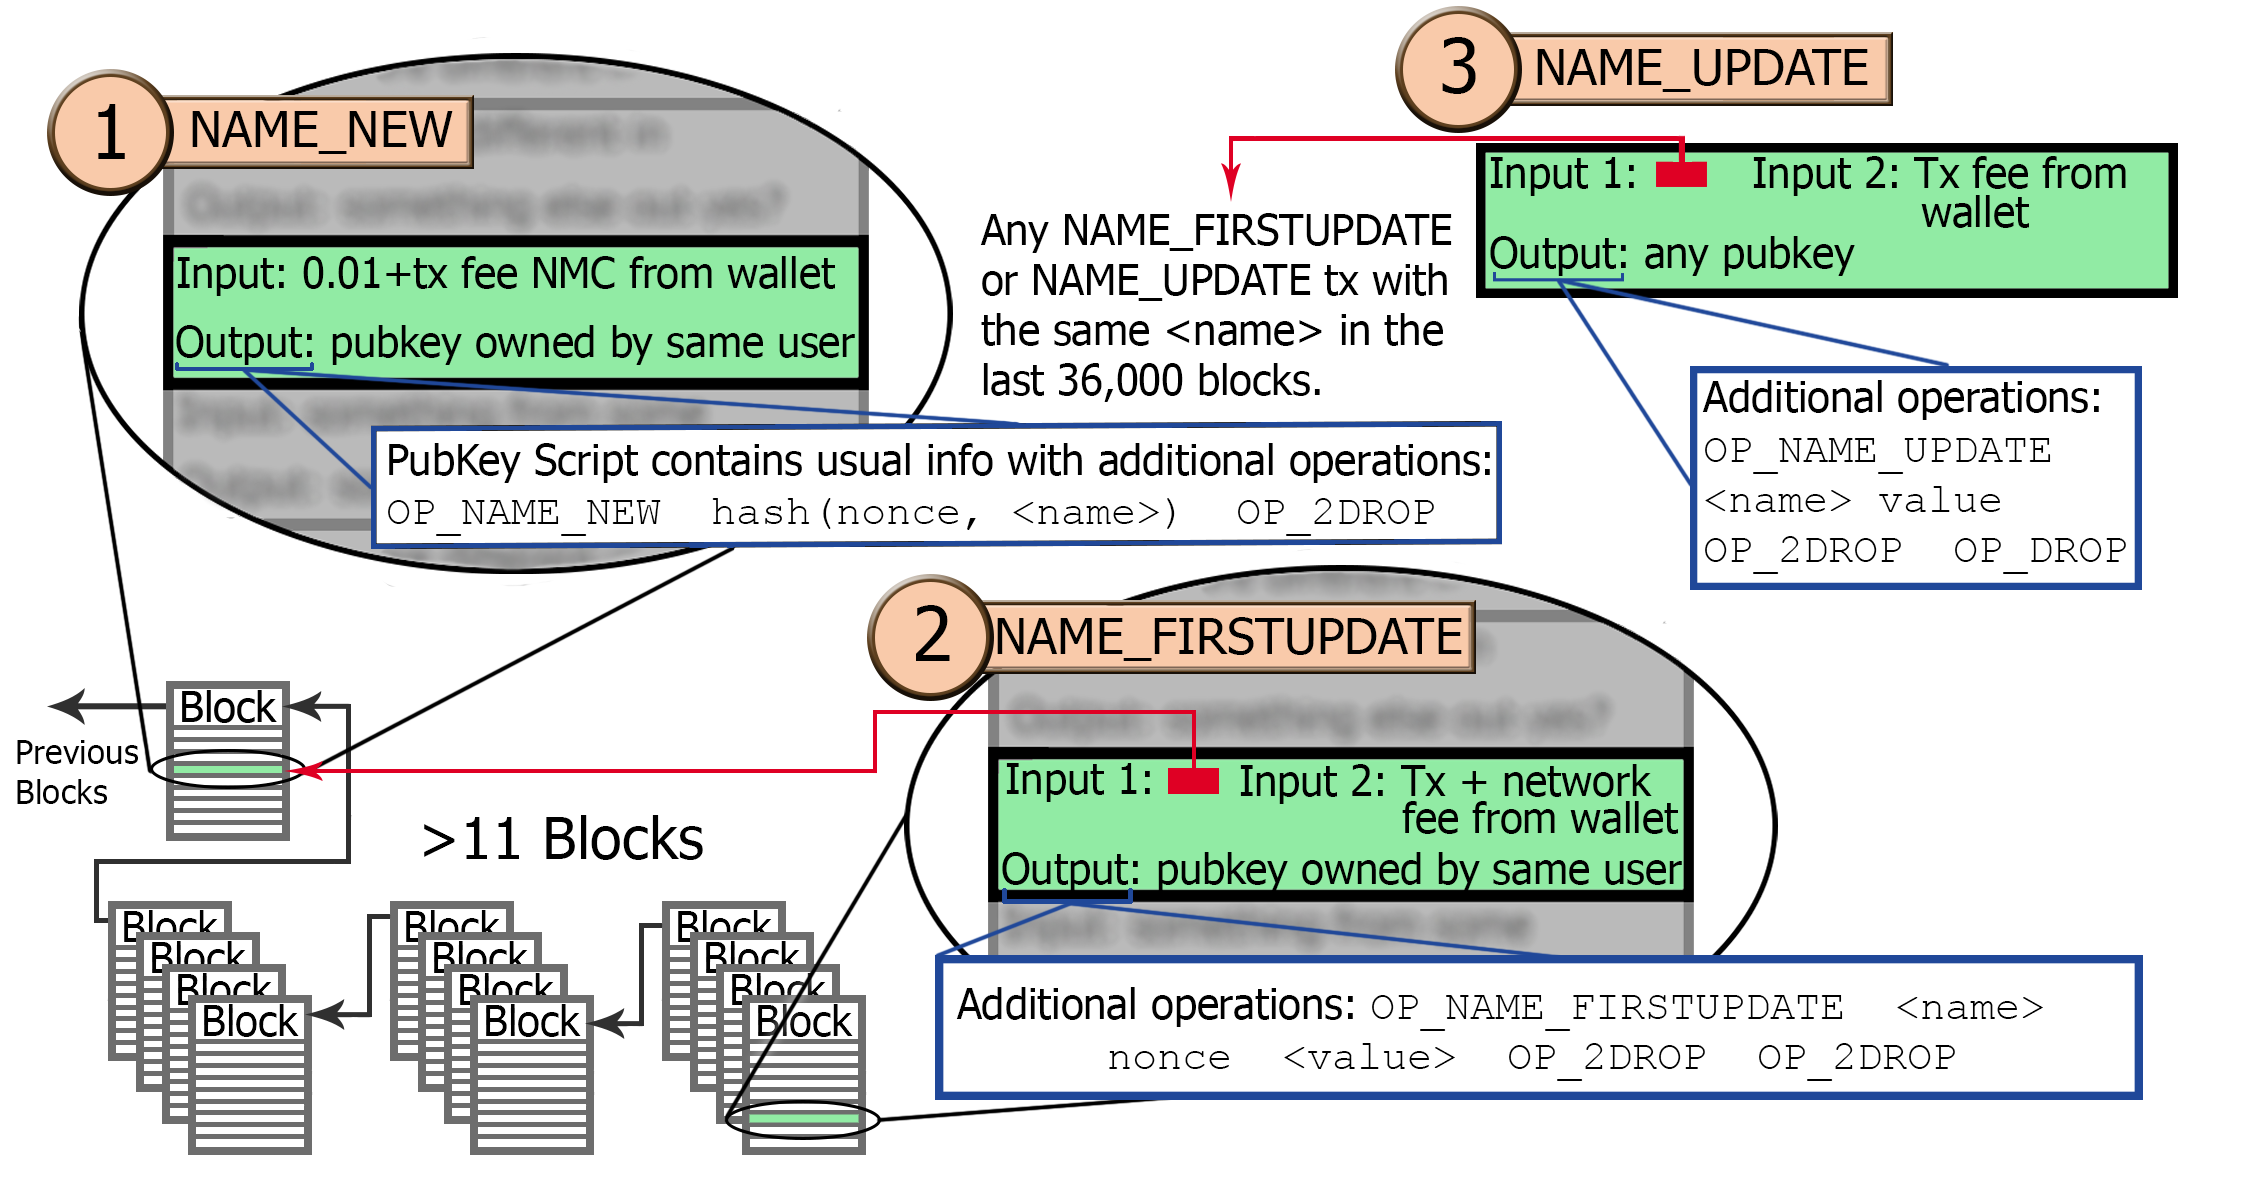
\includegraphics[width=0.95\textwidth]{registration.png}
  \caption{Namecoin Name Registration Protocol}
  \label{fig:registration}
\end{figure*}

 After doing this, and waiting for 12 or more blocks on top of the one containing the NAME\_NEW transaction, the same user can use the output of NAME\_NEW transaction as the input for the NAME\_FIRSTUPDATE transaction. This will now associate the chosen name with a value selected by the user (for example, for use as a distributed DNS, the name would be a d/<name> representing the <name>.bit domain and the <value> would be the location a browser could go to to download the material). Similarly to NAME\_NEW, NAME\_FIRSTUPDATE is posted in the blockchain as part of the scriptPubKey of a special transaction. In addition to using the output from the NAME\_NEW transaction as input, this transaction will also need some additional funds from the users wallet as input to cover the transaction fee and historically a network fee. The network fee is different from the transaction fee; the transaction fee is paid to the miners, whereas the network fee was destroyed when the NAME\_FIRSTUPDATE transaction is confirmed. The network fee varied over time. It started at 50 NMC at the genesis block, but decreased by a factor of 2 every 8192 blocks (which is approximately 2 months). The purpose of the network fee was to have a large initialcost to claiming names to deter users from quickly claiming all the desirable names, but then decay off so that eventually the cost of registering a name becomes negligible. As of block 85585, the network fee became small enough that it rounds to 0 and is no longer added onto the transaction.  As an output of the NAME\_FIRSTUPDATE transaction, the user will again send the special coin to an address they control. The scriptPubKey of the transaction will contain the usual locking script, with the addition of: OP\_NAME\_FIRSTUPDATE, the <name> desired, the random nonce used in the NAME\_NEW operation, the first <value> for the name to take and some additional operations to clear this information from the stack so that they don't interfere with the locking script. In order for this transaction to be valid, a miner will verify that the <name> and the provided nonce do, in fact, hash to the hash in the cited NAME\_NEW transaction. The output of this transaction now contains the token representing the name/value pair, and whoever can unlock and spend the output can utilize the final new operation, NAME\_UPDATE.
The third and final new operation in Namecoin is the NAME\_UPDATE operation. Again, this operation is inserted into the scriptPubKey of a special transaction, along with its arguments (the <name> and <newValue>). This transaction must have as inputs a small fund from the user's wallet (to cover the transaction fee), and a NAME\_FIRSTUPDATE or NAME\_UPDATE output with the same <name> that is less than 36,000 blocks old (which comes out to about 250 days). This operation has two primary uses: the first of which is updating a name, and the second is trading a name. Updating a name can happen for a few reasons. If the user wants to change the value associated with a given name, they will update the name with this operation, providing a new value. The other reason to update is to keep a name fresh, without changing the associated value, so that it can be updated later without violating the 36,000 block age limit. In these cases, the user will use an address they control as an output of the transaction. The other reason to make a NAME\_UPDATE transaction is to trade the special coin to another user. In this case, the user will put, as an output, one of the second user's addresses instead of their own. Once the transaction resolves, the other user will have control over the special coin and can change the value to whatever they deem fit. Because the ownership of a <name> is associated with the ownership of the special coin, if the buyer is paying for the name with Namecoins,  the exchange between the payment and the <name> can be atomic (meaning they happen in the same transaction and either are only valid if the other is as well). If a particular <name> hasn't been mentioned in a NAME\_FIRSTUPDATE or NAME\_UPDATE in 36,000 blocks, the name becomes available again for any user to claim with NAME\_NEW and NAME\_FIRSTUPDATE. 


